\documentclass[border=10pt]{standalone}

\usepackage{tikz}
\usepackage{tikzsymbols}
\usetikzlibrary{calc,patterns,shapes.geometric}

\def\centerarc[#1](#2)(#3:#4:#5){\draw[#1] ($(#2)+({#5*cos(#3)},{#5*sin(#3)})$) arc (#3:#4:#5);}

\begin{document}
	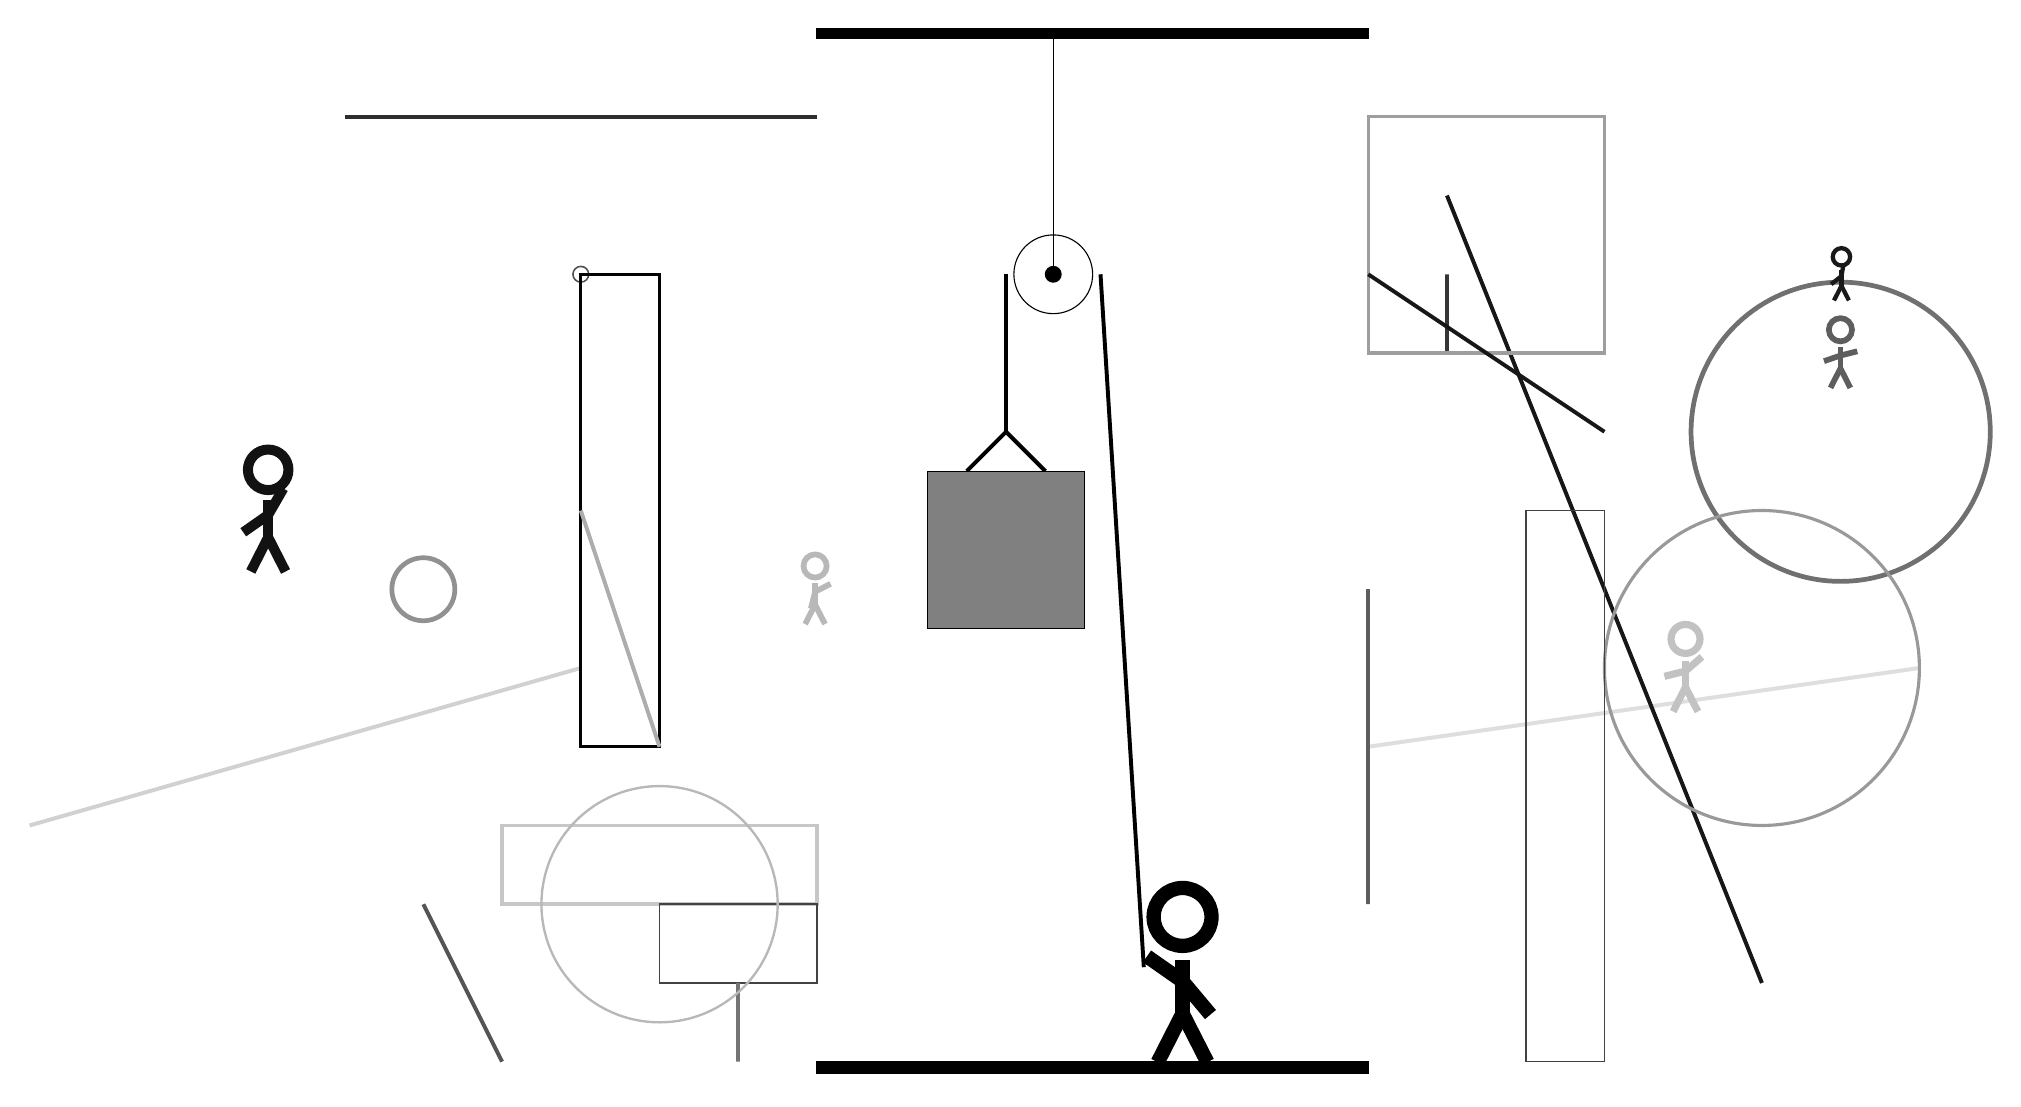
\begin{tikzpicture}
		%%%%% START %%%%%
		
		\draw[fill=black] (-2, 10) rectangle (5, 10.125);
		
		\draw [line width=0.2mm, color=black!69](-5, 7) circle (0.1);
		
		\draw[line width=0.5mm, color=black!22] (-2, 0) rectangle (-6, -1);
		\node[line width=0.2mm, color=black!28] at (-2, 3) {\Strichmaxerl[4][76][27]};
		\draw[line width=0.6mm, color=black!79] (6, 6) rectangle (6, 7);
		\draw[line width=0.5mm, color=black!13](5, 1) -- (12, 2);
		\draw[line width=0.5mm, color=black!18](-5, 2) -- (-12, 0);
		\node[line width=0.7mm, color=black!24] at (9, 2) {\Strichmaxerl[5][14][41]};
		\draw[line width=0.5mm, color=black!63] (5, 3) rectangle (5, -1);
		\draw[line width=0.4mm, color=black!99] (-4, 7) rectangle (-5, 1);
		\draw[line width=0.5mm, color=black!91](6, 8) -- (10, -2);
		\draw[line width=0.5mm, color=black!67](-6, -3) -- (-7, -1);
		\draw[line width=0.2mm, color=black!74] (-4, -1) rectangle (-2, -2);
		\draw[line width=0.3mm, color=black!75] (7, 2) rectangle (7, 0);
		\draw[line width=0.5mm, color=black!82](-2, 9) -- (-8, 9);
		\draw [line width=0.6mm, color=black!56](11, 5) circle (1.9);
		\draw[line width=0.5mm, color=black!54] (-3, -3) rectangle (-3, -2);
		
		\draw [line width=0.6mm, color=black!43](-7, 3) circle (0.4);
		
		\draw[line width=0.4mm, color=black!38] (5, 6) rectangle (8, 9);
		\draw [line width=0.3mm, color=black!28](-4, -1) circle (1.5);
		\draw [line width=0.4mm, color=black!40](10, 2) circle (2.0);
		\draw[line width=0.5mm, color=black!32](-4, 1) -- (-5, 4);
		
		\draw[line width=0.5mm, color=black!91](5, 7) -- (8, 5);
		
		\node[line width=0.3mm, color=black!63] at (11, 6) {\Strichmaxerl[4][19][14]};
		\node[line width=0.5mm, color=black!93] at (-9, 4) {\Strichmaxerl[7][35][60]};
		\node[line width=0.5mm, color=black!90] at (11, 7) {\Strichmaxerl[3][38][80]};
		
		\draw[line width=0.2mm, color=black!74] (7, -3) rectangle (8, 4);
		
		
		\draw (1, 7) circle (0.5);
		\draw[fill=black] (1, 7) circle (0.1);
		\draw (1, 10) -- (1, 7);
		
		\draw[line width=0.5mm] (-0.1, 4.5) -- (0.4, 5.0) -- (0.9, 4.5);
		\draw[fill=black!50] (-0.6, 4.5) rectangle (1.4, 2.5);
		
		\draw[line width=0.5mm] (0.4, 7) -- (0.4, 5.0);
		\centerarc[line width=0.5mm](1, 7)(0:180:0.6);
		\draw[line width=0.5mm](1.6, 7) -- (2.15, -1.8);
		
		\node at (2.6, -1.9) {\Strichmaxerl[10][-35][-50]};
		
		\draw[fill=black] (-2, -3) rectangle (5, -3.15);
		
		%%%%% END %%%%%
	\end{tikzpicture}
\end{document}